\input{/home/nick/latex-preambles/xelatex.tex}

\newcommand{\imagesPath}{.}

\title{
	Αλγόριθμοι και Πολυπλοκότητα \\
	3η σειρά γραπτών ασκήσεων
}
\author{Νικόλαος Παγώνας, el18175}
\date{}

\begin{document}

\maketitle

\section*{Άσκηση 1: Ελάχιστο Συνδετικό Δέντρο με Περιορισμούς}
	\subsection*{(α)}
		Ένα αντιπαράδειγμα που δείχνει ότι το άπληστο κριτήριο δεν λειτουργεί είναι το εξής:
		
		\begin{figure}[H]
			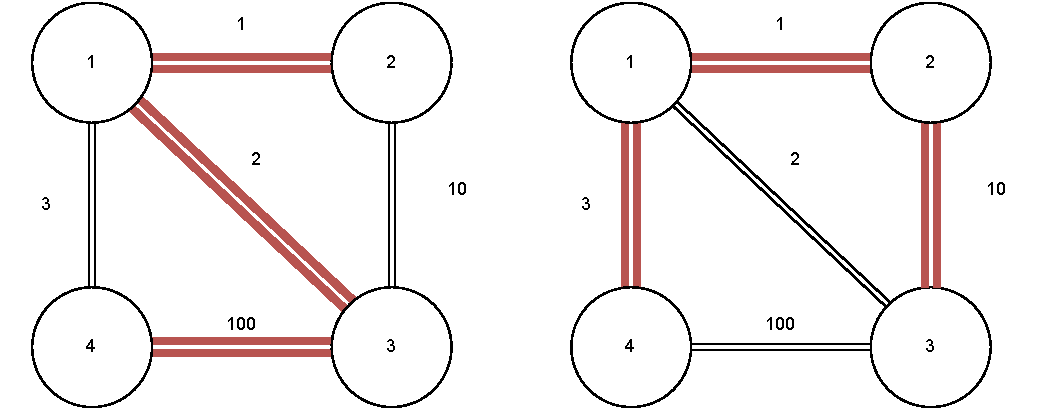
\includegraphics[width=\linewidth]{\imagesPath/counterexample.pdf}
		\end{figure}		
	
		Εδώ απαιτούμε η κορυφή $1$ να έχει βαθμό ίσο με $2$. \\
		
		Το δέντρο που δίνει ο άπληστος αλγόριθμος είναι το αριστερό με βάρος $103$, ενώ το ελάχιστο είναι το δεξί με βάρος $14$.
		
	\subsection*{(β)}
		Η βασική ιδέα είναι η εξής: \\
		
		\begin{itemize}
			\item Προσθέτουμε μία σταθερά $C$ σε κάθε ακμή που προσπίπτει στον κόμβο που μας απασχολεί.
			\item Όσο το $C$ αυξάνεται, τόσο λιγότερες ακμές περιέχει το MST του επαγόμενου γραφήματος που προσπίπτουν σε αυτόν τον κόμβο. 
			\item Εκτελούμε binary search στο $C$.
		\end{itemize}
	
		Αρχικά έχουμε ότι για κάθε απαιτούμενο βαθμό, το MST με περιορισμούς που απαιτείται υλοποιείται ως το MST του δέντρου επαυξημένου κατά $C$. \\
		
		Αυτό ισχύει διότι αν το $C$ είναι αρκετά αρνητικό, τότε το MST λαμβάνει όλες τις σχετικές ακμές, ενώ αν είναι αρκετά θετικό, τότε το MST λαμβάνει τις ελάχιστες δυνατές. Έτσι, όλες οι τιμές μεταξύ της ελάχιστης και της μέγιστης επιτυγχάνονται. \\
		
		Ύστερα έχουμε ότι τα μοναδικά $C$ για τα οποία αλλάζει ο βαθμός του σχετικού κόμβου στο MST είναι αυτά για τα οποία μία ακμή που προσπίπτει στον κόμβο γίνεται ίση με μία άλλη ακμή του γράφου, όταν αυτή αυξηθεί κατά $C$. Συγκεκριμένα, αρκεί να εξετάσουμε τα $C$ που ανήκουν στο σύνολο $S = \{e - d : e \in E \land d \in D\}$, όπου $E$ το σύνολο των βαρών του γραφήματος και $D$ το σύνολο των βαρών ακμών που προσπίπτουν στον κόμβο που μας ενδιαφέρει. \\
		
		Αυτό ισχύει διότι: \\
		Για να βγει μία ακμή από το MST, πρέπει αναγκαστικά να αντικατασταθεί με άλλη. Αυτό σημαίνει ότι για κάποιο $C$, μία ακμή που προσπίπτει στον κόμβο που μας ενδιαφέρει γίνεται ίση με κάποια άλλη ακμή του γραφήματος. Αυτό συμβαίνει μόνο όταν το $C$ είναι ίσο με τη διαφορά μιας ακμής που προσπίπτει στον κόμβο που μας ενδιαφέρει, και μίας άλλης ακμής του γραφήματος. Να σημειωθεί ότι σε κάποιο βήμα υπάρχει το ενδεχόμενο να μπορούν να βγουν πάνω από μία ακμές για το ίδιο $C$. \\
		
		Επομένως ο αλγόριθμος έχει ως εξής: \\
		
		\begin{itemize}
			\item Ταξινομούμε το σύνολο των $C$ που εξετάζουμε, δηλαδή το $S$ (όπως ορίστηκε προηγουμένως), σε χρόνο $O\left(|E||D| \log\left(|E||D|\right)\right)$
			\item Κάνουμε binary search στο $S$. Αυτό γίνεται σε χρόνο $Ο(\log(|E||D|)) = O(\log(|E|))$, αφού $|D| < |E|$. Σε κάθε επανάληψη, προσθέτουμε το συγκεκριμένο $C$ στις ακμές που προσπίπτουν στον κόμβο που μας ενδιαφέρει και εφαρμόζουμε Kruskal (χρόνος $O(|E|\log|E|)$ κάθε φορά). Αυξάνουμε/μειώνουμε το $C$ ανάλογα με το αν ο απαιτούμενος βαθμός είναι αρκετός.  
		\end{itemize}
	
		Ο συνολικός χρόνος είναι $O(|E||D|\log|E| + |E|\log^2|E|)$.
		
\section*{Άσκηση 2: Σχεδιασμός Videogame}

	\subsection*{1.}

		Ο αλγόριθμος έχει ως εξής:
		
		Δημιουργούμε έναν πίνακα $A$ με $n = |V|$ θέσεις, ο οποίος θα περιγράφει την "προσβασιμότητα" κάθε κορυφής. Αρχικά για κάθε κορυφή $u$, έχουμε $A[u] = +\infty$. Στη συνέχεια, για κάθε ακμή $(u, v)$: \\
		
		Ελέγχουμε αν $A[v] > A[u] + p(v)$ και $A[u] + p(v) > 0$ (ο "χειρότερος" τρόπος που μπορεί να φτάσει -ζωντανός- ο παίκτης στο δωμάτιο $v$, αν μπορεί να φτάσει καν). Αν ισχύουν οι παραπάνω συνθήκες, τότε ο παίκτης μπορεί να πάει από το δωμάτιο $u$ στο δωμάτιο $v$ και να του μείνει ενέργεια ίση με $A[u] + p(v) > 0$, οπότε ανανεώνουμε $A[v] = A[u] + p(v)$. \\
		
		Στο τέλος της επανάληψης ελέγχουμε αν $A[t] > 0$ και $A[t] \neq +\infty$. \\
		
		\textbf{Χρονική πολυπλοκότητα:} 
		Η πολυπλοκότητα του αλγορίθμου είναι $O(|V|\cdot|E|)$, γιατί η αρχικοποίηση του πίνακα $A$ χρειάζεται $O(|V|)$, ενώ ο έλεγχος που κάνουμε για κάθε ακμή θα εκτελεστεί το πολύ $|V|$ φορές (επειδή έχουμε υποθέσει πως δεν έχουμε κύκλους), επομένως συνολικά η επανάληψη κοστίζει $O(|V|\cdot|E|)$
		
	\subsection*{2.}
		
		Εκτελούμε και πάλι την διαδικασία του (1), και ελέγχουμε αν $0 < A[t] \neq +\infty$. Αν όχι, τότε εκτελούμε άλλο ένα iteration της διαδικασίας και αν κάποια από τις τιμές του πίνακα αλλάξει, αυτό σημαίνει πως έχουμε κύκλο θετικού μήκους, στον οποίο μπορούμε να φτάσουμε από την $s$ με αρχική ενέργεια $r$. Αφού ανακαλύψουμε ότι υπάρχει κύκλος θετικού μήκους που πληροί τις παραπάνω προδιαγραφές, δεν μας ενδιαφέρουν πλέον τα βάρη, γιατί μπορούμε να διανύσουμε όσες φορές θέλουμε τον κύκλο και να πάρουμε όση ενέργεια μας χρειάζεται για να ολοκληρώσουμε τη διαδρομή μέχρι την κορυφή $t$. Με DFS μπορούμε εύκολα τόσο να βρούμε τους κύκλους, όσο και να ελέγξουμε αν η $t$ είναι προσβάσιμη από κορυφές του κύκλου. Ακόμα και να εκτελέσουμε DFS για όλες τις κορυφές, η χρονική πολυπλοκότητα δεν αλλάζει σε σχέση με πριν, άρα έχουμε $O(|V|\cdot|E|)$.

	\subsection*{3.}

		Για να βρούμε το ελάχιστο $r$ εφαρμόζουμε την γνωστή διαδικασία μετατροπής προβλήματος απόφασης σε πρόβλημα βελτιστοποίησης, δηλαδή κάνουμε δυαδική αναζήτηση στο $r$, και για το εκάστοτε $r$ τρέχουμε τον παραπάνω αλγόριθμο.

\section*{Άσκηση 4: Επαναφορά της Ομαλότητας στη Χώρα των Αλγορίθμων}

	Για να λύσουμε το πρόβλημα θα το ανάγουμε σε πρόβλημα εύρεσης μέγιστης ροής. \\
	
	Κατ' αρχήν, κάνουμε την εξής παρατήρηση: \\
	Για να αιχμαλωτίσει έναν Εξτρεμιστή ή να κλείσει μία βάση, το ελάχιστο κόστος για τον στρατό είναι να εκμεταλλευτεί τον στρατιώτη που βρίσκεται πιο κοντά. \\
	
	Έτσι, δημιουργούμε ένα γράφημα (έστω $G$) που έχει $n_E$ κόμβους αφιερωμένους στους Εξτρεμιστές, $n_B$ κόμβους αφιερωμένους στις βάσεις και $2$ επιπλέον βοηθητικούς κόμβους $v_1$, $v_2$, επομένως έχουμε συνολικά $n_E + n_B + 2$ κόμβους. Ο σκοπός μας είναι να ενώσουμε κάθε κόμβο-Εξτρεμιστή με κάθε κόμβο -βάση από την οποία η απόστασή του είναι μικρότερη ή ίση του $d$. Για το σκοπό αυτό, ξεκινάμε με άπειρη χωρητικότητα σε κάθε τέτοια ακμή. Επίσης, ενώνουμε κάθε κόμβο-εξτρεμιστή με τον κόμβο $v_1$ και θέτουμε ως χωρητικότητα την απόσταση του κοντινότερου στρατιώτη σε αυτόν. Αντίστοιχα ενώνουμε κάθε κόμβο-βάση με τον $v_2$ και πάλι έχουμε χωρητικότητα την απόσταση του κοντινότερου στρατιώτη σε αυτόν.\\
	
	Στην συνέχεια παρατηρούμε ότι το $v_1 - v_2$ Min Cut είναι το κόστος που αναζητούμε. (επειδή έχουμε άπειρα κόστη μεταξύ εξτρεμιστών και βάσεων, το min cut θα περιέχει ακμές από το $v_1$ σε κόμβους-εξτρεμιστές και από το $v_2$ σε κόμβους-βάσεις). \\
	
	Είναι εύκολο να βρούμε το Min Cut, βρίσκοντας το αντίστοιχο Max Flow (πχ με Ford-Fulkerson). \\
	
	Για το $G$, αρχικά ταξινομούμε στρατιώτες, βάσεις και εξτρεμιστές με βάση την απόστασή τους από το $0$ σε χρόνο $O(N \log N)$, όπου $N = n_S + n_B + n_E$, ($n_S$ ο αριθμός των στρατιωτών) οπότε το $G$ φτιάχνεται πλέον σε γραμμικό χρόνο. \\
	
	Κυρίαρχος όρος της πολυπλοκότητας του αλγορίθμου είναι το κόστος του Max Flow αλγορίθμου (πχ με βελτιώσεις Edmonds-Karp $O(|V|^2\cdot|E|)$).


\section*{Άσκηση 5: Αναγωγές και NP-Πληρότητα}
	\subsection*{Τακτοποίηση Ορθογωνίων Παραλληλογράμμων}
		Θα κάνουμε αναγωγή από το 2-Partition. \\
		
		\textbf{Βασικό σκεπτικό:} Έστω τα ορθογώνια $A_i$ με μεγέθη $a_i \cdot ε$ ($ε < 1$, μπορεί να επιλεγεί κατάλληλα). Έστω επίσης $B$ το μεγάλο ορθογώνιο που έχει μέγεθος $s \cdot 2ε $. Η ιδέα είναι να επιλέξουμε $s = \frac{1}{2}\sum_{i}a_i$. Έτσι, αν μπορούμε να τοποθετήσουμε τα $n$ ορθογώνια μέσα στο $B$ τότε, λόγω του πλάτους του θα είχαμε κάνει partition το σύνολο ${a_1, ..., a_n}$ σε δύο σύνολα ίδιου μεγέθους. Βέβαια, για να δουλέψει αυτό θα πρέπει να επιλέξουμε σωστά το $ε$ προκειμένου να μην επιτρέψουμε περιστροφές στην τοποθέτηση των $A_i$. 
			
	\subsection*{Μέγιστη Τομή με Βάρη στις Κορυφές}
	
		Αφού για κάθε $v \in V$ έχουμε $w(v) \geq 1$, έχουμε ότι, αν μπορέσουμε να βρούμε μία διαμέριση $(S, V \textbackslash S)$ των κορυφών $V$ της κλίκας τουλάχιστον βάρους $B$, τότε: 
		
		\[
			B \leq w(S, V \textbackslash S) = \sum_{u \in S, v \notin S} w(u) \cdot w(v) = \sum_{u \in S} w(u) \cdot \sum_{v \in [n] \textbackslash S} w(v) 
		\]
		
		Η τελευταία ισότητα προκύπτει γιατί έχουμε για γράφημα μια κλίκα. \\
		Στην συνέχεια, παρατηρούμε τα εξής: 
		
		\begin{itemize}
			\item Το πρόβλημά μας είναι πολυωνυμικά ισοδύναμο με το να μεγιστοποιήσουμε το βάρος της τομής (απλά αντί να έχουμε στόχο το $B$, δουλεύουμε στην κλάση NPO).
			\item Αν A = $\sum_{i \in [n]}w(i)$, τότε το δεξί μέλος της παραπάνω ανισότητας έχει τη μορφή:
				\[
					w(S)(A-w(S)) \leq A^2/4
				\]
				
				Η ανισότητα αυτή προκύπτει επειδή η συνάρτηση $x\cdot(C-x)$ μεγιστοποιείται στη θέση ${x = C/2}$.
		\end{itemize}
	
		Επομένως, μπορούμε να χρησιμοποιήσουμε το 2-Partition. Αν είχαμε ένα σύνολο με θετικούς ακεραίους και θέλαμε να το διαμερίσουμε σε δύο ισοβαρή υποσύνολα, τότε, με βάση τα παραπάνω, αρκεί να μεγιστοποιήσουμε την τομή ενός γραφήματος με κορυφές όσες και ο πληθάριθμος του 2-Partition στιγμιοτύπου, και βάρη στις κορυφές ίσα με τα στοιχεία του συνόλου που μας δίνεται.
	
	\subsection*{Συντομότερο Μονοπάτι με Περιορισμούς (Constrained Shortest Path)}
		Θα κάνουμε αναγωγή από το Knapsack. \\
		
		Στο Knapsack έχουμε $n$ στοιχεία, με βάρη $w_i$ και κέρδη $p_i$, και ρωτάμε αν υπάρχει κάποιο υποσύνολό τους με συνολικό βάρος $\leq B$ και συνολικό κέρδος $\geq P$. \\ 
		
		Δημιουργούμε ένα (κατευθυνόμενο) γράφημα με κορυφές $v_0, ..., v_n$ όπου $v_0$ η αρχική κορυφή και $v_1, ..., v_n$ αντιστοιχούν σε στοιχεία του σακιδίου. Βάζουμε δύο κατευθυνόμενες ακμές από κάθε $v_{i-1}$ στο $v_i$. Η μία ακμή αντιστοιχεί στην επιλογή του στοιχείου $i$, οπότε θα έχει μήκος $w_i$ και κόστος $P_{\text{sum}} - p_i$, όπου $P_{\text{sum}} = \sum_{i} p_i$. Η άλλη ακμή αντιστοιχεί στην μη-επιλογή του στοιχείου και θα έχει μήκος 0 και κόστος $P_{\text{sum}}$. Θέτουμε $s = v_0, \ t=v_n, \ W=B \ \text{και} \ C=n\cdot P_{\text{sum}} - P$. \\
		
		Φαίνεται εύκολα ότι η εύρεση σακιδίου είναι ισοδύναμη με την εύρεση έγκυρου μονοπατιού.  
\end{document}